%%%%%%%%%%%%%%%%%%%%%%%%%%%%%%%%%%%%%%%%%%%%%%%%%%%%%%%%
%%%
%%%  LaTeX template for InTech Journal article
%%%
%%%  IMPORTANT NOTICE:
%%%  Due to the double blind peer review process, 
%%%  make sure to omit the author information from the manuscript. 
%%%  You will be asked to enter these information separately during author
%%%  registration in InTech MTS system.
%%%
%%%  Submitted content will be processed through XML workflow, so 
%%%  final PDF will not be generated from this LaTeX template.	
%%%
%%%%%%%%%%%%%%%%%%%%%%%%%%%%%%%%%%%%%%%%%%%%%%%%%%%%%%%%

\documentclass{intech-journal}


%%%%%%%%%%%%%%%%%%%%%%%%%%%%%%%%%%%%%%%%%%%%%%%%%%%%%%%%
%%% 
%%%  Note that amsfonts,amstext,amssymb,amsmath,amsthm,amscd
%%%  bm,paralist,color,graphicx,array and subfigure packages
%%%  are all part of intech-journal.cls
%%%  Please avoid using additional packages.
%%%
%%%%%%%%%%%%%%%%%%%%%%%%%%%%%%%%%%%%%%%%%%%%%%%%%%%%%%%%




\articletitle{R2T2 : Robotics to Integrate Educational Efforts in South Africa and Europe } % To break lines in long titles use \\


\begin{document}
\maketitle

\articleabstract{}
\keywords{Rescue, Educational Robotics, Thymio robot, Space Robotics, Programming}

\section{Introduction}
The South African government is working at improving Science, Technology, Engineering and Mathematics (STEM) interests within schools for scholars to become excited with these careers that are limited in the country. 
As mechatronics engineering and robotics are the integration of mainly mechanical, electronic and computer engineering disciplines, it allows for the skills in these areas to be learned. 

Different factors have an influence of scholar's learning activities within Africa, which include toilet facilities, building infrastructure, computer equipment facilities and laboratories,  libraries, and learning teaching support~\cite{sedibe2011inequality}. Furthermore, poverty, poor housing, inadequate skills development, lack of energy sources, inadequate drinking water and sanitation, poor communications, poor education and training, lack of transport, lack of sporting and recreational activities and cultural deprivations, are only a few factors that have created disadvantaged scenarios, of which Apartheid is often to be blamed~\cite{mokoena2009improving}. Yet, after 21 years after Apartheid, there is not necessarily an improvement in these conditions, but often a degrees in the improvements of the conditions.

Many of the above mentioned problems are vastly related to the lack of engineering skills. Improving on these skills, especially which correlate with mechanical, electronic and computer engineering, can allow many people to improve their living conditions. Many times these living conditions can be improved on by a person who have the interest to learn and solve their problems. It has been evident of such scenarios with people in Malawi who have no education, yet were able to learn the skills and thus allow themselves to build windmills, as a means to generate electricity and pump water~\cite{Sheerin2009}.

With the use of Robotics, South Africa has pursued education events such as the First Lego League South Africa~\cite{FLLSA}, First Tech Challenge South Africa~\cite{FTCA}, the World Robotics Olympiad~\cite{WRO}, and participation to the RoboCup Junior contest~\cite{ferrein2011robocup}. 
Sadly these activities and events are often pursued with the upper-class schools, who have the computer facilities, an internet connection, and teachers who have been enthusiastic to educate the students with resources above those in the normal syllabus. 
For instance some scholars are able to attend robotics at the Cape Town Science Center as an extra mural activity, yet payment is required to be made to attend these sessions [e]. 

These events are organized also in Europe, rising some similar issues but in another context.
Robot competitions, in Europe, attract only participants already interested in STEM topics, and have very few impact on most people~\cite{riedo2013upgrade}.
Moreover very few women are participating in these events, contributing to a gender gap on education about technology~\cite{riedo2013upgrade}.
In some extent the elitist aspect of these competitions is similar to South Africa, even if expressed differently.

Another common characteristic of the existing events is that they are all based on competitive activities. 
Existing surveys suggest that collaborative activities could motivate a larger public~\cite{riedo2013upgrade}.

To summarize, both in South Africa and Europe it is hard to bring robotics into schools, for different reasons. 
In South Africa the economic factor plays a more important role, but the European comfort of the teachers is also a barrier to changes.
In both realities it would be interesting to have activities that generate a broader interest, better motivate the teachers, can reacher a broader public and are economically affordable.

The Thymio II robot has been indicated as an appropriate robotic platform to pursue STEM in Africa~\cite{Gyebi2015}, as it is an open source platform with a sensory system that include a microphone, IR proximity sensors, temperature sensor, odometer and accelerometers, with the use of open source programming language, Aseba~\cite{magnenat2010aseba}. 
The Thymio robot has been broadly spread in schools in Europe\cite{roy2015inirobot}, and used as a tool for teaching many topics, from physics~\cite{Mubin2013} to computer science~\cite{magnenat2014}. 
Even though the Thymio robot has been one of the more expensive educational robots that have been used in Africa~\cite{Gyebi2015}, it has been cheaper than the Lego Mindstorm EV3 robots, and it has been one of the best robots with processing, sensors, deployment, development and maintenance.
 
This paper presents an education activity addressing the issues above by using the opportunity offered by the Thymio robot. 
In opposition to the existing events, it focus on a collaborative task, based on a rescue operation.
To gain attractiveness, the rescue scenario is set on a mars station. 
This scenario allows to add and justify an important aspect: the delay of transmission of the video. 
This delay is necessary for ensuring the video streaming but is also realistic in respect to the operation on Mars.
Moreover this delay excludes the possibility to remote control the robots, forcing the participants to program them.
Finally the rescue scenario requires the coordination of 16 teams controlling 16 robots, and therefore allows to include in the event other activities different than programming: coordination in the team and with other teams, communication, planning, validation of distant results, etc.
This broad spectrum of activities enable the inclusion of teachers from various disciplines and participants with different interests.

After this introduction, the next section introduces the event.....XXXXX


\section{State of the art}
%(a) existing platforms and (b) initiatives in (South) Africa
\paragraph{Technologies in Education \cite{winthrop2012new}}

\paragraph{Potential of robots in classroom}
Usage in STEM

\paragraph{Competitions and challenges}

\paragraph{Summer camps}

\paragraph{Existing robotics platform in stem education \cite{Karim2015}}
Table with existing platform
\begin{table*}[h]
\begin{tabular}{|c|c|c|c|c|c|} \hline
Name & Education Level & Open & Hardware & Programming & Dispersion \\ \hline

\end{tabular}
\caption{}
\end{table*}

what are the initiatives in Africa and other south countries

table of paper talking abut initiatives


\section{Thymio and the R2T2 initiative}

\begin{figure*}[ht]
 \centering
    \includegraphics[width=\columnwidth]{figures/setup-schematic.pdf}
  \caption{Infrastructure of the R2T2 experiment.}
  \label{fig:setup-scheme} 
\end{figure*}

\begin{figure*}[ht]
 \centering
    \includegraphics[height=45mm]{figures/setup.pdf}
    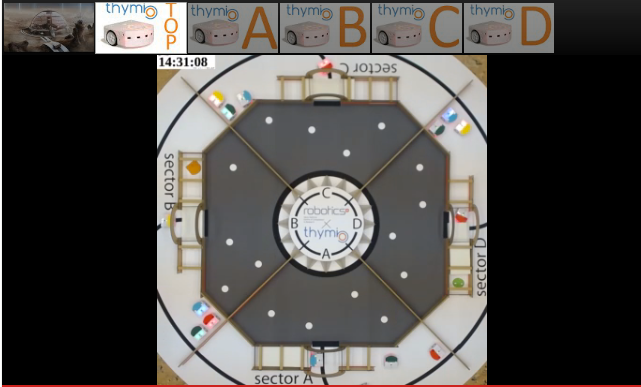
\includegraphics[height=45mm]{figures/youtube-view.png}
  \caption{Physical setup in EPFL Lausanne and view of the station on YouTube.}
  \label{fig:setup-physical} 
\end{figure*}


\section{Survey among the children}: results

\section{Discussion and conclusion}
Government schools in South Africa did not readily offer French as a language course and a high profile secondary school was therefore selected for participation in the event, in order to meet the requirements of having at least one team member who was fluent in French. The theme of the event attracted the top students from various grades within the selected school. These students formed the team that participated in the event and all students in the team had prior experience with programming and hobby kits such as the Arduino Uno programmable controller. 
The training of the team was made easier due to the fact that the selected students had prior programming knowledge. A set of instructions was supplied with the Thymio kit along with a training manual which introduced the user to the various functions and capabilities of the robot. The method used to train the students involved implementation of the training manual and this was supplemented with allocating tasks specific to the environment in which the team worked. Table … lists the progression of the training performed with the students. This progression followed the installation of the software onto the individual stations used by the students. The team was given a set of four robots and an additional robot for the teachers to experiment with. 

\begin{table}
\centering
\caption{Progression of the training performed on selected South African students}
\begin{tabular}{|p{5cm}|p{5cm}|p{5cm}|} \hline
Task from training manual & Supplementary task & Observation of students \\\hline
N/A &  Introduction to programming methodology: Students were taken through the process of deconstructing a program into logic, pseudocode and then implementation of relevant programming language. A task was allocated to the team to list the pseudocode and draw a flowchart for the processes associated with making a cup of coffee. Students were then asked to attempt to make the cup of coffee using the instructions they provided. &
Students were already exposed to programming and assumed that this was a redundant step. Students found that they could not successfully complete the task when following their own instructions. The reason for the failure was due to the lack of consideration and blatant ignorance of the exact steps required to fulfil the task. \\\hline
Introduction to programming environment: This step introduced students to the concept of using a visual programming interface as opposed to a text based interface.  &
None &
Students were excited by the ease with which the robot could be programmed using a visual interface. They had only been exposed to text based programming and the graphical representation of functions was welcomed. \\\hline
Introduction to events and the robotic platform &
Students were asked to perform actions based on a command as if they were the robot. This allowed the team to identify the relation between the events and the resulting actions. Students were then asked to associate colours with moods. &
Students viewed the platform as a toy initially. This encouraged them to approach the use of the platform in a jovial manner as they were not intimidated by the complex system that lay within the platform. Most of the students associated red with danger and green with a pleasant robot state.  \\\hline
Moving the robot : Students were required to move the robot back and forth &
A task was given to students to move the robot around the table on which they worked. This task exposed them to open loop control of the platform. &
Students ensured that they provided a flowchart and relevant pseudocode for the robot operation in order to complete the task. It was noticed that they showed enthusiasm in testing their predetermined values and make the necessary adjustments in order to follow the path around the desk. It was at this stage that the students started to display intense focus. \\\hline
Using the sensors and using states in advanced mode: Students were required to explore the capabilities of the sensory capabilities of the robot. They were required to implement a program that would allow the robot to exhibit the behaviour of a pet. This behaviour relied on the use of states in the advanced mode. &
The team was also given the task of programming the robot to behave in the fashion that their personal pets would.  &
Students took more time in completing this task due to the complexities associated with the safety considerations such as ensuring the robot did not fall off the table. Four unique behaviours were observed which included exploratory behaviour, aggressive behaviour and seemingly irrational behaviour (which students insisted was in accordance with the behaviour of their animals). \\\hline
Use of range of values and angle options: Students had to experiment with using a range of values for the sensors. &
A track was built and robots were required to accelerate uphill and decelerate downhill. Obstacle avoidance was also required.  &
Students had no problem in implementing the code once their logic and pseudocode was implemented. \\\hline

\end{tabular}

\end{table}



It was also observed that the initial team of four members had expanded to twelve as the initial team took it upon themselves to train their peers who showed interest. 

The R2T2 event required a lot of preparation. Except that the equipment had to be setup for the event, the communication and streaming of video was challenging, due to the limited internet bandwidth. At the South African event were two YouTube video streams (https://www.youtube.com/watch?v=sd3tdzocsFY and https://www.youtube.com/watch?v=q5NX98K2ptg), which was very choppy and the sound was not streamed and recorded properly, due to the limited bandwidth. More video streaming were considered, but were cancelled when it was realized that the YouTube footage was not recorded properly.

The two YouTube streams from EPFL, which represented the Mars environment and the scenario, were projected, one being the global view, and the other being the specific sector view (Sector D). The delays of the videos that were created at EPFL, to represent the delay in communication between Mars and Earth, was very interesting in the way that the participants had to plan the challenges. The participants often wanted to stop the robot, but then the instruction would take time before the robot received it. In saying this, it was observed that the YouTube stream from EPFL had an additional lag, due to the limited bandwidth. Viewing the same video stream through a smartphone and a GPRS signal, showed different video footage and were thus out of sync. This was challenging for the participants as the video feedback and thus the robot response was not consistent.

The participants thought that they could give the Thymio robot instructions and get things working the first time, even though they were advised not to do so. They learned very quickly to follow the advice, and to work in a team, to first simulate instruction on the robot they had within the lab, before sending the instruction to the robot. After the participants changed their approach, it indicated that they were more successful with attempting the challenges. 

There was a problem experienced with the communication with the Thymio robot form South Africa, in that the robot did not respond to instructions. The reason for the malfunction is uncertain, yet after numerous attempts to send the instruction, and realizing that the robot did not perform after the expected delay in transmission, the connection was reset by EPFL.

The participants were frustrated at times when things did not happen as they expected, yet once they realized that they had to solve the problems using smaller steps and in a sequential manner, it showed to be more successful. It has been found to be the most challenging aspect with the teaching of robotic systems within South Africa, with the sequential steps in the programming of the robots. It is found that the scholars are able to grasp the mechanical component quite easily, as they have been exposed to building structures, whether it is with sand, stones, sticks, or even more advanced material such as building bricks, Lego blocks or metal materials. The understanding of the electronic component is grasped a little more difficult, yet with the scholars being exposed to more electronic systems and being taught electrical circuits from a young age, they are able to connect the different components and modules together. The aspect that scholars have difficulty with is the programming. Even though they are taught of planning with flowcharts and pseudocode, and indicated that they must think of themselves being the robot and the steps that is needed to be followed, the scholars have a difficulty with sequential instructions. There are many factors for the scholars to have a difficulty to understand this concept, and it could be due to everything happening lately automatically, with less problem solving, as technology has developed, and also due to scholars not being exposed to programming at a younger age. Typically, within South Africa, some scholars are only exposed to programming for the first time in grade 8, otherwise only in grade 10 should they have taken computer science as a secondary school subject. It has also been found that some students are only exposed to programming when they reach university level, as their school did not have computer facilities and limited technology equipment. It is believed that this hurdle will only be overcome once programming skills are to be taught from the beginning of the scholar’s school career, which can be pursued with activities such as placing the sequence of event into order with the different activities they need to perform to get to school every morning. Similar activities will make the scholars to have a better understanding with sequential programming in the future.


\bibliography{r2t2}{}

\end{document}